
%Remove these comments at end if they are fulfilled

% Before you begin, make sure that:
% - research question is clear
% - main points(contribution)+goal are clear (to be repeated throughout+title)
% - clear validation, evaluation, method of exactly the research question with main points as outcome!!!
% - Brainstorming was done
% - Roter Faden was done (Strukturierung und Elimination of Abzweigung)

\documentclass[12pt]{report}
\usepackage[utf8]{inpute nc}
\usepackage[acronym,nomain]{glossaries}
\usepackage{cite}
\usepackage{hyperref}
\usepackage{tcolorbox}
\usepackage{graphicx}
\usepackage{subcaption}
\usepackage[section]{placeins}

\title{Viability of TOML parsing for configuration}
\author{Jakob Fischer}


\bibliographystyle{unsrt}
\makeglossaries

\newacronym{ll}{LL}{Left-to-Right, Leftmost derivation}
\newacronym{lr}{LR}{Left-to-Right, Rightmost derivation}
\newacronym{toml}{TOML}{Tom's Obvious, Minimal Language}
\newacronym{flex}{Flex}{Fast Lexical Analyzer}
\newacronym{posix}{POSIX}{Portable Operating System Interface}

\newcommand{\onlinesrc}[1]{Accessed #1}
\newcommand{\gitsrc}[1]{Commit \##1}

\begin{document}

\maketitle

\begin{abstract}
TODO: Abstract
\end{abstract}

\chapter{Introduction}


\section{\acrshort{toml}}
\acrlong{toml} (\acrshort{toml}) is a configuration file format developed since February, 2013 \cite{tomlcontrib}.
It claims to be a format, that is easily to read and parse \cite{tomlreadme} and finds use in many different projects \cite{tomlwiki}.
For instance, it is used with Rust's project manager \textbf{cargo} \cite{cargogit}, as well as Python's package installer \textbf{pip} \cite{piprefguide}.

\section{Elektra}
Elektra is a configuration framework for accessing configuration settings in a global key database \cite{Elektramain}.
An application using Elektra can read and write key/value pairs via calls to the Elektra library, making the implementation of an own configuration system obsolete.
Furthermore, elektrified applications can access configuration settings of other elektrified applications, to provide better application interoperability.

Although Elektra is mainly written in C, there are bindings for other languages like java, python or ruby \cite{Elektrabindings}.

Elektra can also read from and write to different configuration file formats, like JSON, XML or ini \cite{Elektrastorage}.
If the need arises, applications can easily switch to a different file format, because configuration access is done with the Elektra API.
Developers or Administrators no longer need to commit to one file format for configuration.

Support for different languages and file formats is implemented by the use of plugins, which can be enabled if needed.
With this modularity, Elektra can provide a wide range of functionality, while simultaneously avoiding being a bloated library.
Developers can compile Elektra with the exact set of needed functionality. If they don't need bindings for java, they can just disable this feature.

\section{LCDproc}
LCDproc is an open source project for displaying stats like CPU/RAM usage of a system on different kinds of LCD devices \cite{LCDprocmain}\cite{LCDprocgit}.
It has a client/server architecture, where the clients provide their system stats to the server, which can display them on a LCD device.

\section{Research Question}
We will test the newly written toml plugin on ElektraInitiative's fork of LCDproc, where LCDproc is currently in the process of using Elektra for it's handling of configuration.
The toml plugin will be used as the storage plugin for the LCDproc configuration.
We will create a \acrshort{toml} configuration file based LCDproc's main configuration file for evaluation.

There are three questions we want to answer for the toml plugin:
\begin{itemize}
	\item[\textbf{RQ1}] Does the plugin correctly read the LCDproc configuration?
	\item[\textbf{RQ2}] Does the plugin correctly write the LCDproc configuration without any loss of information?
	\item[\textbf{RQ3}] Does the plugin put an unreasonable overhead on LCDproc loading times?
\end{itemize}
Ad RQ1 we must ensure, that were are really reading the configuration from our supplied file, and not the default values supplied by the Elektra specification.

Ad RQ2 we also have to check, if comments and newlines - which don't affect the LCDproc execution practically, but are only for the user to read - are preserved.

\chapter{Implementation}

The plugin is implemented in C, using the C99 standard. It requires \acrshort{posix} for it's capabilities to check regular expressions.

\section{Plugin}
The toml parser is realized as an Elektra storage plugin. The plugin exposes two functions, \textbf{ElektraTomlGet} for reading, and \textbf{ElektraTomlSet} for writing, as expected of a storage plugin.

\section{Tools}
It uses two external tools for generating a parser for the toml file format: \textbf{\acrshort{flex}} \cite{flexgit} for lexical analysis and \textbf{bison} \cite{bisonmain} for parsing.
The key generation is done in the bison parser with the use of actions.

In order to generate the appropriate Elektra keys, the parser has access to a driver which contains all needed Elektra logic.
We oriented on the existing Elektra plugin \textbf{yambi}\cite{Elektrayambi} in key generation via driver.
The driver contains functions of the style \textbf{driverEnterKey}/\textbf{driverExitTable}, to make it more clear at what point of parsing a certain function shall be invoked.

\section{Grammar}
Since bison generates \acrshort{lr} (\acrlong{lr}) parsers, grammar rules should be be left-recursive.
Otherwise, we could run out of stack memory, if recursing too deep with a right-recursive rule.
The created parser only contains left-recursive rules.
TODO: Maybe explain better/examples/sources

The parser makes use of so-called midrule-actions, which are parser actions that are not at the end of a grammar rule.
This can affect the resulting grammar, since after executing a mid-rule action, the parser has to commit to the chosen parse branch \cite{bisonmidruleconflicts}.
We tried to minimize the usage of midrule-actions, to make the grammar as independent of actions as possible.
However, especially for possibly nested structures, like arrays or inline tables, they were unavoidable.

\chapter{Evaluation}

\section{Hardware Setup}
The evaluation was executed on the following hardware setup:
\begin{verbatim}
Processor: Intel i7-4790K @ 4.20 GHz
RAM: 16 GB (2 x 4GB, 1 x 8GB), DDR-3 @ 1600 MHz 
HDD: Seagate Desktop ST2000DM001, 2TB, 6 GB/s
\end{verbatim}

\section{Software Setup}

The following versions of Elektra and LCDproc were used for evaluation:
\begin{tcolorbox}
\begin{verbatim}
Elektra:
repository: github.com/bauhaus93/libelektra.git
branch: 'plugin_toml'
commit: #e75d60f8699d8ea80f0f099364b3b8f03ec4413f
LCDproc:
repository: github.com/bauhaus93/lcdproc.git
branch: 'toml_test'
commit: #70bf70135190c270c6a75e0b975f591df323bb65
\end{verbatim}
\end{tcolorbox}


The evaluation was done within a docker container, which was built as follows.
\begin{tcolorbox}
\begin{verbatim}
cd libelektra
docker build -t buildElektra-buster \
    --build-arg JENKINS_USERID=`id -u` \
    --build-arg JENKINS_GROUPID=`id -g` \
    -f scripts/docker/debian/buster/Dockerfile \
    scripts/docker/debian/buster/
\end{verbatim}
\end{tcolorbox}

We extended this image by building another image on top of it. This dockerfile mainly installs/sets up sudo for installing Elektra and LCDproc.
Dockerfile:
\begin{tcolorbox}
\small
\begin{verbatim}
FROM buildelektra-buster

USER root
RUN apt-get update && apt-get -y install sudo vim tmux
RUN adduser jenkins sudo
RUN echo '%sudo ALL=(ALL) NOPASSWD:ALL' >> /etc/sudoers
USER jenkins
WORKDIR /home/jenkins
\end{verbatim}
\end{tcolorbox}

From our working directory within the container, Elektra and LCDdproc get installed with another script:
\begin{tcolorbox}
\small
\begin{verbatim}
./lcdproc/toml_setup_install.sh
\end{verbatim}
\end{tcolorbox}

Since the default configuration LCDd file is very minimal, and most of the configuration is loaded by the specification, we created a LCDd \acrshort{toml} file for evaluation purposes.
It is based on the old default configuration file of LCDd \cite{LCDprocconf}.
We converted this old configuration from it's ini like format into \acrshort{toml}.
All driver configuration settings, which are not referenced in the specification \cite{bauhaus93forklcdprocslcddspec}, were removed from it.
To show the full capability of the parser, the syntax of the following lines was changed into a semantically equivalent format:
\begin{verbatim}
[menu]
menukey = "Escape"
enterkey = "Enter"
upkey = "Up"
downkey = "Down"
\end{verbatim}
was changed into an inline table:
\begin{verbatim}
menu = { menukey = "Escape", enterkey = "Enter", \
		 upkey = "Up", downkey = "Down" }
\end{verbatim}

The resulting \acrshort{toml} file has 606 lines including 369 lines of comments and 143 empty lines.
It contains one \acrshort{toml} table, nested array and inline table.
It contains multiple \acrshort{toml} table arrays - one for each driver.

This file is copied to our configuration directory in \texttt{.config/} by our installation script.
It is also mounted as configuration file for LCDd by the post-install.sh script, used in the installation script.

We force a full read/write roundtrip of the configuration file, by setting the currently used driver. This driver is already the active driver in the file, but we set it again.
Afterwards, we check if there are any differences between the original file and the newly written file.
The executed diff command ignores any differences in whitespace, since whitespace are yet only preserved before comments by the plugin (tabs are normalized to 4 spaces).
{\small
\begin{verbatim}
kdb set '/sw/lcdproc/lcdd/#0/current/server/drivers/#0' '@/curses/#0'
diff -ws ./lcdproc/LCDd.toml .config/LCDd.toml
Files ./lcdproc/LCDd.toml and .config/LCDd.toml are identical
\end{verbatim}
}
After one roundtrip, the resulting LCDd.toml is identical to the original file under disregard of whitespace.
\\\\

\section{LCDd}
We start and stop the LCDd daemon once, change some parameters of the curses driver, and start the daemon again.
{\small
\begin{verbatim}
LCDd -f
kdb set '/sw/lcdproc/lcdd/#0/current/curses/#0/foreground' 'yellow'
kdb set '/sw/lcdproc/lcdd/#0/current/curses/#0/background' 'blue'
kdb set '/sw/lcdproc/lcdd/#0/current/curses/#0/backlight' 'blue'
kdb set '/sw/lcdproc/lcdd/#0/current/curses/#0/size' '100x40'
LCDd -f
\end{verbatim}
}

The resulting output of LCDd is:
\FloatBarrier
\begin{figure}[h!]
	\centering
	\begin{subfigure}[b]{0.4\linewidth}
		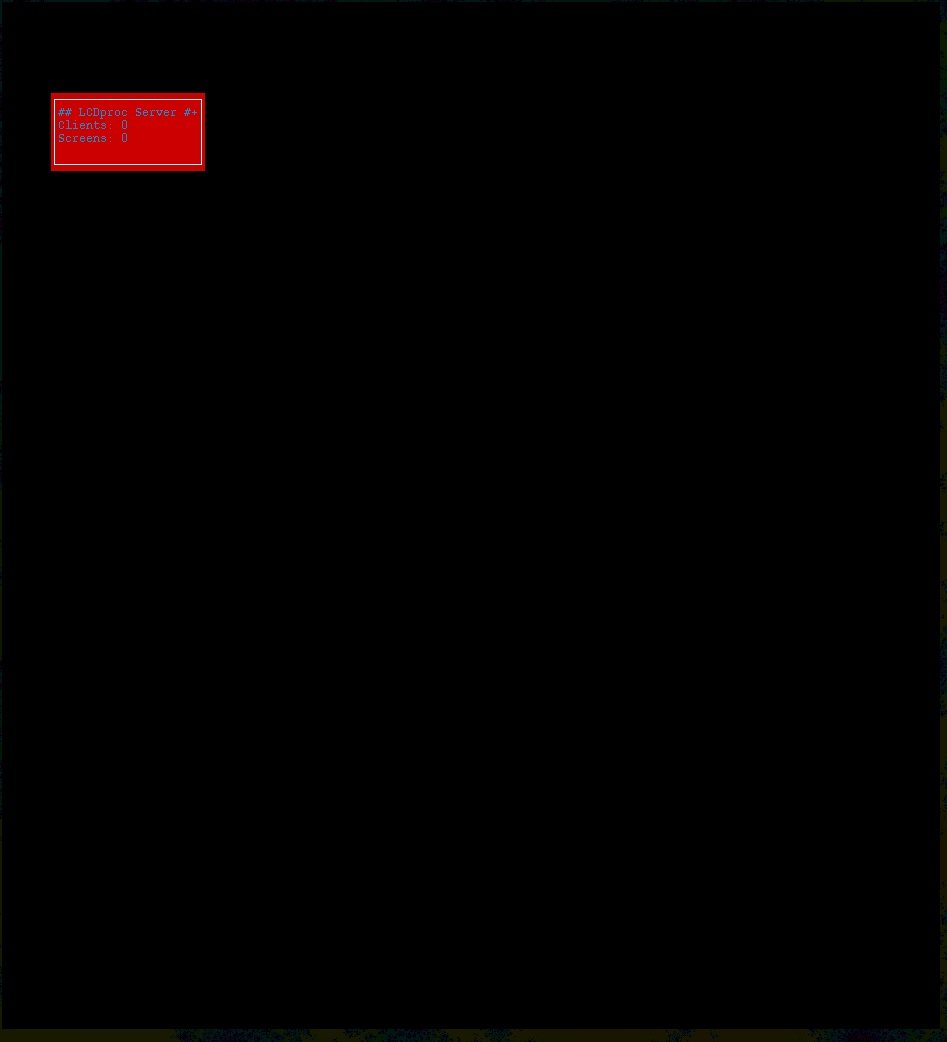
\includegraphics[width=\linewidth]{lcdd_vanilla.png}
		\caption{Before parameter change}
	\end{subfigure}
	\begin{subfigure}[b]{0.4\linewidth}
		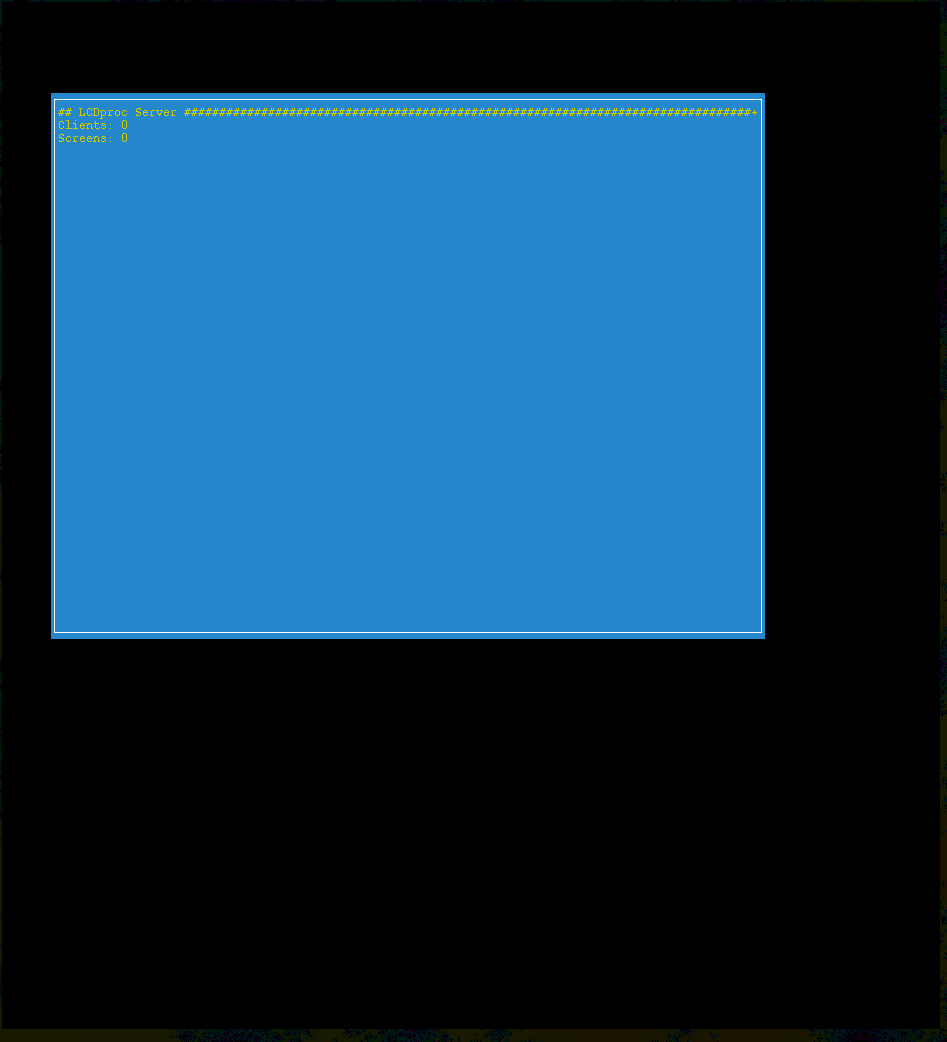
\includegraphics[width=\linewidth]{lcdd_changed.png}
		\caption{After parameter change}
	\end{subfigure}
  \caption{LCDd output}
\label{fig:lcdd}
\end{figure}
\FloatBarrier
We observe, that we successfuly changed the foreground/background color and window size of the daemon.

\section{lcdproc}
The lcdproc configuration gets roundtripped by changing the used port from the file default of 13666 to 12345.
Afterwards the file difference without whitespace get checked.
{\small
\begin{verbatim}
kdb set 'user/sw/lcdproc/lcdproc/#0/current/lcdproc/port' '12345'
diff -w ./lcdproc/lcdproc.toml .config/lcdproc.toml
9c9
< port=13666
---
> port = 12345
\end{verbatim}
}
The only difference found is the line with the port number, for which we changed the value.
The rest of the file remained unchanged.
\\\\
Then, the lcdproc client gets started without an active LCDd-daemon.
{\small
\begin{verbatim}
lcdproc -f
sock_connect: connect failed
Error connecting to LCD server localhost on port 12345.
Check to see that the server is running and operating normally.
\end{verbatim}
}
In the error message, we see that the client tried to connect to port 12345, and not the default 13666.




\section{Benchmarks}


\chapter{Related Work}

\chapter{Conclusion}

\chapter{Glossary}

\printglossary[type=\acronymtype]

\bibliography{references}{}
\bibliographystyle{plain}

\end{document}
